
\section{M/G/1}


Se trata de un sistema de líneas de espera con un solo servidor en el que los tiempos entre llegadas son exponenciales, pero la distribución de los tiempos de servicio no requiere ser exponencial.

Definimos

\begin{center}
$\frac{1}{\mu}=E(S)$ y   $\sigma^2= Var(S)$
\end{center}

Observamos que este modelo no es un proceso de nacimiento-muerte ya que los tiempos de servicio no tienen la propiedad de carencia de memoria de la exponencial, y la probabilidad de que el servicio se complete entre $t$ y $t + \Delta t$ cuando el estado del sistema en el tiempo $t$ es $j$ depende del tiempo transcurrido desde que se completó el último servicio.\\

Determinar las probabilidades de estado estable no es una tarea sencilla debido a que ya no son válidas las ecuaciones de estado estable en el proceso de nacimiento-muerte.

Para ello, utilizamos los resultados de Pollaczek y Khinchin para determinar $L_q$, $L$, $L_s$, $W_q$, $W$, $W_s$. Pollaczek y Khinchin demostraron que para un sistema de colas de este tipo

\begin{equation}
L_q=\frac{\lambda^2 \sigma^2+\rho}{2(1-\rho)}
\end{equation}

donde $\rho=\displaystyle\frac{\lambda}{\mu}$. Como $W_s=\displaystyle\frac{1}{\mu}$, por las fórmulas de Little se tiene que $L_s=\lambda\left(\displaystyle\frac{1}{\mu}\right)=\rho$. Como $L=L_s+L_q$ obtenemos que

\begin{equation}
L=L_q+\rho
\end{equation}

Nuevamente de las fórmulas de Little tenemos

\begin{equation}
W_q=\frac{L_q}{\lambda}\\
W=W_q+\frac{1}{\mu}
\end{equation}

		\begin{figure}[h]
			\centering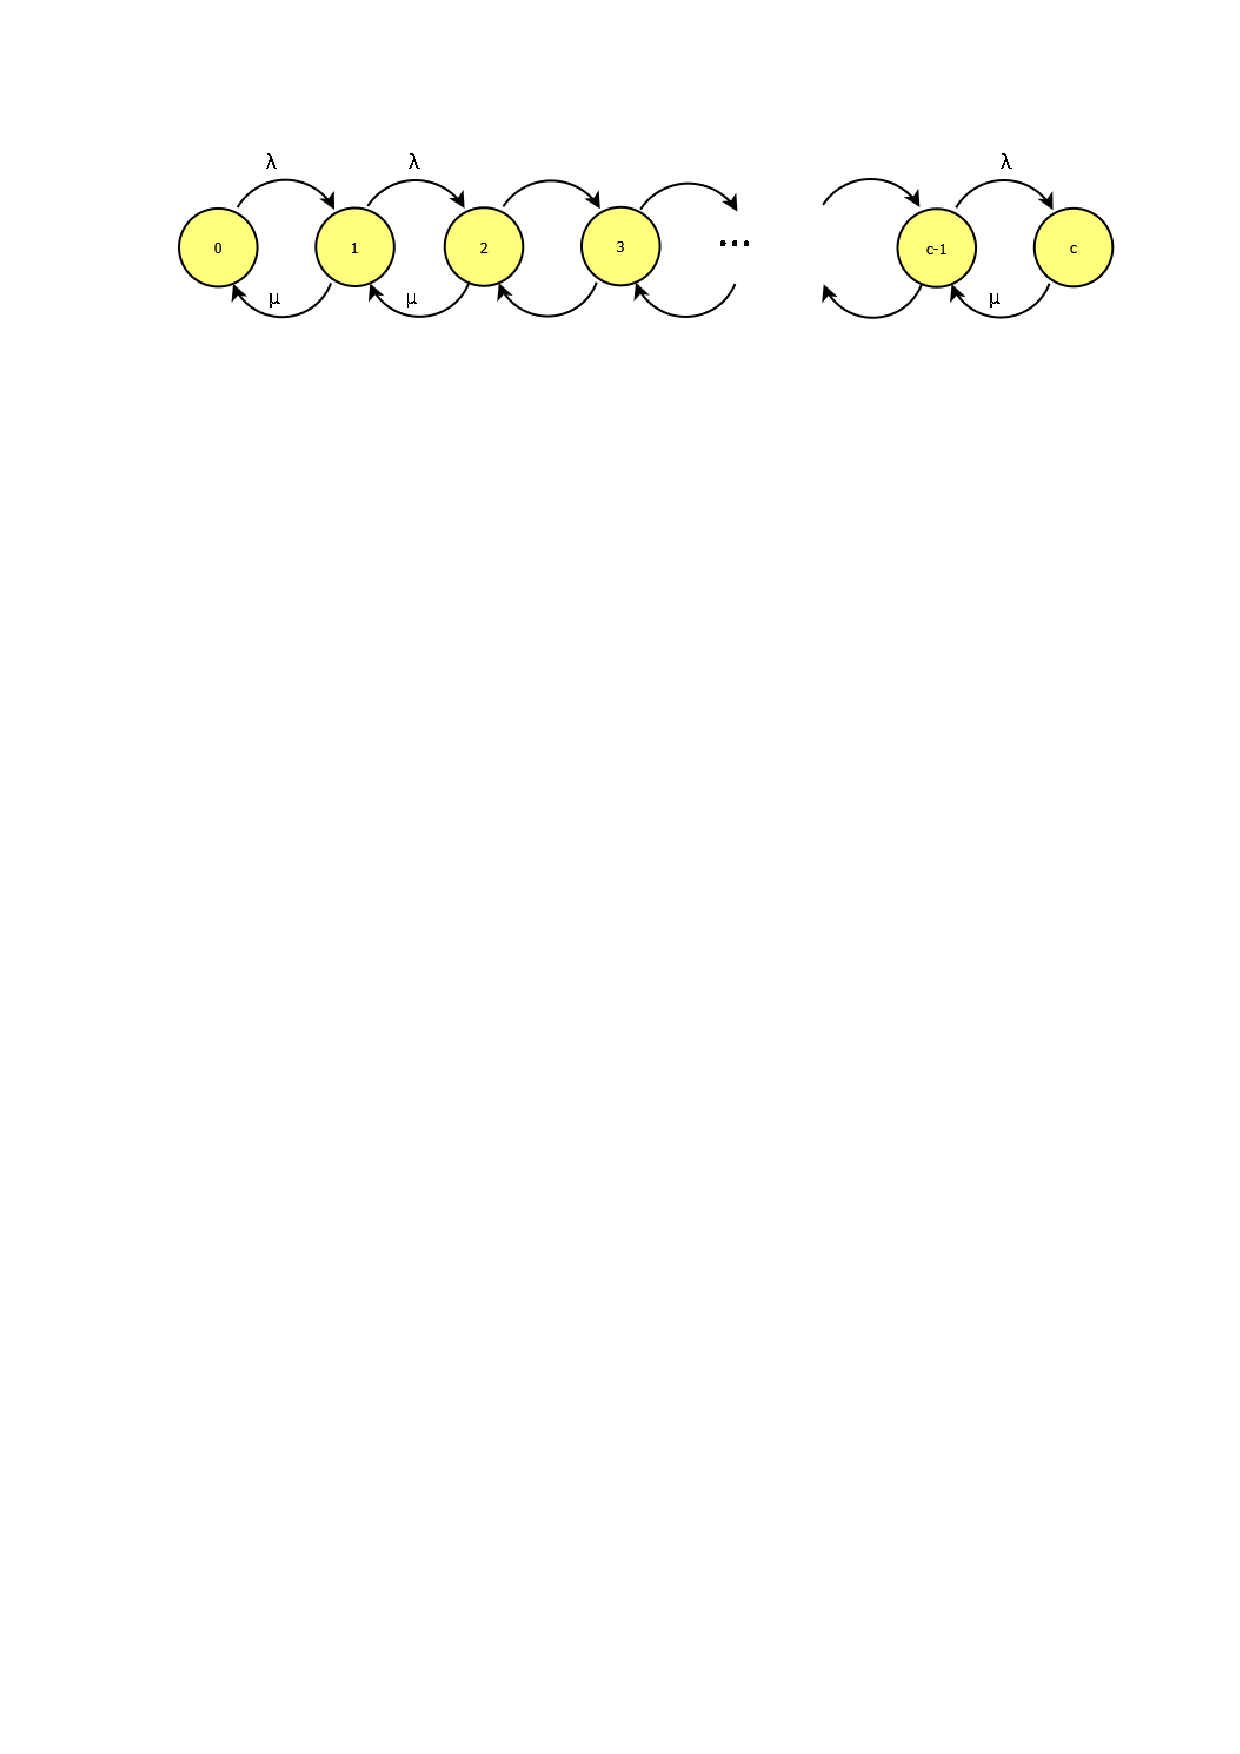
\includegraphics[trim = 10mm 220mm 10mm 25mm, clip,width=0.9\linewidth]{MMc}
		\end{figure}
		

